\documentclass[journel,12pt,twocoloums]{IEEEtran}

\title{Assignment 6-Probability and Random Variable}
\author{Annu-EE21RESCH01010}
\date{13 January 2020}

\usepackage{amsthm}
\usepackage{graphicx}
\usepackage{mathrsfs}
\usepackage{txfonts}
\usepackage{stfloats}
\usepackage{pgfplots}
\usepackage{cite}
\usepackage{cases}
\usepackage{mathtools}
\usepackage{caption}
\usepackage{enumerate}	
\usepackage{enumitem}
\usepackage{amsmath}
\usepackage[utf8]{inputenc}
\usepackage[english]{babel}
\usepackage{multicol}
%\usepackage{xtab}
\usepackage{longtable}
\usepackage{multirow}
%\usepackage{algorithm}
%\usepackage{algpseudocode}
\usepackage{array,multirow}
\usepackage{enumitem}
\usepackage{mathtools}
\usepackage{gensymb}
\usepackage{hyperref}
%\usepackage[framemethod=tikz]{mdframed}
\usepackage{listings}
    %\usepackage[latin1]{inputenc}                                 %%
    \usepackage{color}                                            %%
    \usepackage{array}                                            %%
    \usepackage{longtable}                                        %%
    \usepackage{calc}                                             %%
    \usepackage{multirow}                                         %%
    \usepackage{hhline}                                           %%
    \usepackage{ifthen}                                         %%
  \providecommand{\nCr}[2]{\,^{#1}C_{#2}}
  \providecommand{\nPr}[2]{\,^{#1}P_{#2}}
  \lstset{
%language=C,
frame=single, 
breaklines=true,
columns=fullflexible
}

 \begin{document}
 \maketitle
\textbf{Download latex code from here-}\\
\begin{lstlisting}
 https://github.com/annu100/AI5002-Probability-and-Random-variables/tree/main/ASSIGNMENT_6
 \end{lstlisting}
 \textbf{download python code from here}\\
 \begin{lstlisting}
  https://github.com/annu100/AI5002-Probability-and-Random-variables/blob/main/ASSIGNMENT_5/assignment_6.py
 \end{lstlisting}
 \section{Problem Statement-Problem 5.19}
 A carton consists of 100 shirts of which 88
are good, 8 have minor defects and 4 have
major defects.Jimmy, a trader, will only accept
the shirts which are good, but Sujatha, another
trader, will only reject the shirts which have
major defects.One shirt is drawn at random
from the carton. \\\ What is the probability that 
(i) it is acceptable to Jimmy?
(ii) it is acceptable to Sujatha?
Also generate random variables according to 3 categories i.e good shirts,minor defect shirts and major defect shirts.
\section{SOLUTIONS}
\subsection{Probability calculation}
\begin{table}[ht]
\caption{Given data-table}
\begin{center}
\begin{tabular}{|p{4cm}|p{4cm}|}
\hline
\multicolumn{2}{|c|}{\textbf{Total number of shirts =100}}\\ \hline \hline
\multirow{2}{*}{88 good shirts} & out of 100, 88 are good shirts

\\
\hline
\multirow{2}{*}{8 Number of minor defected  } & out of 100,8 are accepted minor defected shirts\\ \hline
\multirow{2}{*}{4 Number of minor defected } & out of 100,4 are accepted major defected shirts\\ \hline
\hline
\end{tabular}
\end{center}
\end{table}
Total number of shirts =100\\ 

Number of good shirts =88\\

Number of minor defected shirts =8\\

Number of major defected shirts =4\\


(1) Acceptable shirts to jimmy =88\\

required probability =$\frac{88}{100}$\\


 =0.88\\
(2) Acceptable shirts to sujata =88+8=96\\

required probability =$\frac{96}{100}$\\

 =0.96\\
 \subsection{Random numbers generation}
 \begin{table}[ht]
\caption{Random variables}
\begin{center}
\begin{tabular}{|p{4cm}|p{4cm}|}
\hline
\multicolumn{2}{|c|}{\textbf{A Random variable which has 3 possible vales}}\\ \hline \hline
\multirow{2}{*}{Pr_(X=0)=\frac{4}{100}=004} & out of 100, 4 have major defects shirts

\\
\hline
\multirow{2}{*}{Pr_(X=1)=\frac{8}{100}=0.08} & out of 100,8 are accepted minor defected shirts\\ \hline
\multirow{2}{*}{Pr_(X=0)=\frac{88}{100}=0.88} & out of 100,88 are accepted good shirts\\ \hline
\hline
\end{tabular}
\end{center}
\end{table}
 let numtrials is sample size
 p is 3 length vector containing probabilities(pmf)
 X is random variable which has 3 outcomes
p=[0.04,0.08,0.88]\\Given distribution P(X=0)=0.04 ,P(X=1)=0.08 ,P(X=2)=0.88
Now generating numtrials samples according to given probability distribution described in above table.\\

Generated samples according to the probability distribution is 

['2', '2', '2', '1', '0', '2', '2', '2', '2', '2', '2', '2', '2', '2', '2', '2', '2', '2', '2', '1', '1', '2', '2', '2', '2', '2', '2', '2', '0', '2', '2', '2', '0', '2', '2', '2', '2', '2', '2', '2', '2', '2', '2', '2', '1', '2', '2', '2', '2', '2', '2', '2', '1', '1', '2', '2', '2', '2', '1', '1', '2', '2', '2', '2', '1', '2', '2', '2', '2', '2', '2', '2', '2', '2', '1', '0', '2', '2', '2', '2', '2', '2', '2', '2', '2', '2', '2', '2', '2', '2', '2', '2', '1', '2', '2', '2', '2', '2', '2', '2']\\
\\
\\
Actual probabilities are [0.04, 0.08, 0.88] \\
simulation probabilities are given by \\
Probability for X=0 is  0.04 \\
Probability for X=1 is  0.11 \\
Probability for X=2 is  0.85 \\
\\
\\
\begin{figure}
\caption{grapgh for actual probability versus simulated probability}
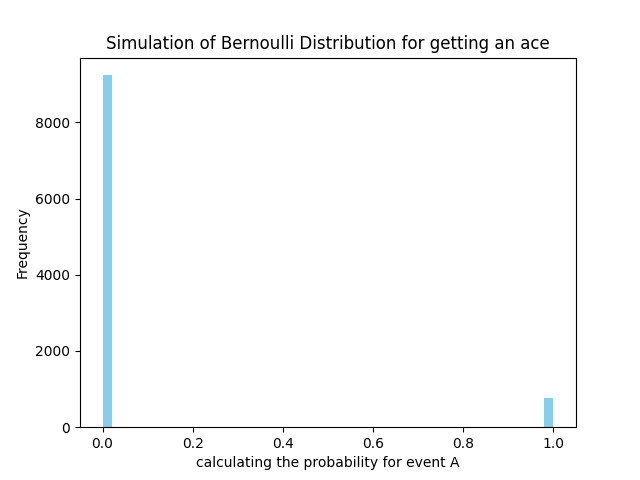
\includegraphics[width=\columnwidth] {Figure_1.png}
\textbf{Above is is the grapgh for actual probability versus simulated probability and we can see almost they are same}\\
\end{figure}

\end{document}

        

